\section{Definizione di processi di Markov}%
\label{sub:Lezione 4}
\mylocaltoc
\subsection{Processi stazionari e processi di Markov}%
\label{sub:Processi stazionari e processi di Markov}
\subsubsection{Probabilità di un processo}%
\label{subsub:Probabilità di un processo}
Prendiamo un oggetto vittima di un processo stocastico dipendente dal tempo e mettiamoci in un sistema di coordinate spaziali $x$. \\
Possiamo descrivere completamente il processo con la sequenza di $P_n$ definite come:
\[
    P_n(x_1,t_1; x_2,t_2; \ldots ; x_n,t_n) 
.\] 
Ovvero la densità di probabilità che l'oggetto si trovi in $x_1$ al tempo $t_1$, $x_2$ al tempo $t_2$ etc\ldots \\
Per descrivere il moto non basta la densità di probabilità allo step $n$-esimo ma serve l'intera sequenza $P_1, P_2, \ldots$\\
Scegliamo una base spazio temporale ($\overline{x} = (x,t)$), le proprietà delle $P_n$ sono:
\begin{itemize}
    \item $P_n \ge 0$.
    \item Simmetria: $P_n(\overline{x}_1;\overline{x}_2; \ldots) = P_n(\overline{x}_2; \overline{x}_1)$.
    \item Completezza:
	\[
	    \int P_n(\overline{x}_1;\ldots;\overline{x}_n) dx_n = P_{n-1}(\overline{x}_1;\ldots;\overline{x}_{n-1}) 
	.\] 
    \item Norma: $\int P_1(\overline{x}_1) dx_1 = 1$ 
\end{itemize}
Possiamo calcolare il valor medio di una quantità nel seguente modo:
\[\begin{aligned}
    &\left< x(t_1) \cdot \ldots \cdot x(t_n) \right> =\\
			     & \qquad=\int\limits_{R^n} dx_1\ldots dx_n P_n(\overline{x}_1;\ldots ;\overline{x}_n) x_1 \ldots x_n
.\end{aligned}\]

\begin{greenbox}{Processi stazionari}
    Un processo si dice stazionario se $\forall n$:
    \[\begin{aligned}
	P_n&(x_1,t_1;\ldots;x_n,t_n) =\\
	=&P_n(x_1,t_1+\Delta t;\ldots;x_n,t_n+\Delta t)
    .\end{aligned}\]
\end{greenbox}
\noindent
\subsubsection{Probabilità condizionata}%
\label{subsub:Probabilità condizionata}
Ipotizziamo che all'istante $t_i$ l'oggetto si trovi in $x \in \left[x_i, x_i + \Delta x\right]$ (con $i \in \left[1, k\right]$).\\
Allora la probabilità che l'oggetto si trovi in un istante successivo $t_{k+l}$ in un intervallo $\left[x_{k+l}, x_{k+l} + \Delta x\right]$ è:
\[\begin{aligned}
    P_{k+l}&(\overline{x}_1;\ldots; \overline{x}_{k+l}) =\\
    =&P_k(\overline{x}_1;..;\overline{x}_k)\cdot P_{l|k}(\overline{x}_{k+1};..;\overline{x}_{k+l}|\overline{x}_1;..;\overline{x}_k) 
.\end{aligned}\]
Con $P_{l|k}$ probabilità di trovarsi in un intorno di $x_{k+l}$ condizionata dai primi $k$ step. 
\begin{exmp}[Prob. condizionata dal primo step]
    Ipotizziamo di avere la probabilità di essere in $x_1$ al tempo $t_1$, vogliamo trovare la probabilità di essere in $x_2$ al tempo $t_2$:
    \[
	P_2(\overline{x}_1;\overline{x}_2) = P_{1|1}(\overline{x}_2|\overline{x}_1) \cdot P_1(\overline{x}_1) 
    .\] 
\end{exmp}
\noindent

\begin{greenbox}{Processi di Markov}
    Un processo si dice Markoviano se le sole conoscenze di $P_1$ e di $P_{1|1}$ sono sufficienti per studiare l'intera evoluzione del processo.
    \[
	P_{1|n-1}(\overline{x}_n|\overline{x}_1;\ldots;\overline{x}_{n-1})  = P_{1|1}(\overline{x}_n|\overline{x}_{n-1}) 
    .\] 
\end{greenbox}
\noindent
Fisicamente un processo di questo tipico indica che il sistema è senza memoria.

%%%%%%%%%%%%%%%%%%%%%%%%%%%%%%%%%%%%%%%
%  Equazione di Chapman - Kolmogorov  %
%%%%%%%%%%%%%%%%%%%%%%%%%%%%%%%%%%%%%%%

\subsection{Equazione di C-K}%
\label{sub:Equazione di Chapman-Kolmogorov}
L'equazione di Chapman-Kolmogorov si applica ai processi Markoviani. Si parte dalla seguente identità:
\[
    \sum_{B}^{\Omega} P(A \cap B \cap C) = P(A \cap C) 
.\] 
Per un processo Markoviano (con ordinamento $t_1 < t_2 < t_3$) l'equazione per la $P_3$ è:
\[
    P_3(\overline{x}_1; \overline{x_2}; \overline{x}_3) = P_{1|1}(\overline{x}_3| \overline{x}_2) P_{1|1}(\overline{x}_2 | \overline{x}_1) 
    P_1(\overline{x}_1) 
.\] 
Integrando rispetto alla coordinata $x_2$ e sfruttando la completezza delle $P_n$ si ha:
\[
    \int P_3(\overline{x}_1; \overline{x_2}; \overline{x}_3) dx_2 = P_2(\overline{x}_1;\overline{x}_3) = P_{1|1}(\overline{x}_3|\overline{x}_1) P_1(\overline{x}_1)
.\] 
Mettendo tutto insieme e semplificando ambo i lati la $P_1(\overline{x}_1)$:
\begin{redbox}{Equazione di Chapman-Kolmogorov}
    \[\begin{aligned}
	P_{1|1}(x_3|x_1) = \int P_{1|1}(x_3|x_2) P_{1|1}(x_2|x_1)dx_2 \label{eq:3_CK}
    .\end{aligned}\]
\end{redbox}
\noindent
Quindi un processo Markoviano rispetta l'equazione di Chapman-Kolmogorov, tuttavia non vale il viceversa!
\subsection{Continuità dei processi stocastici}%
\label{sub:Continuità dei processi stocastici}
\begin{defn}[Processo continuo]
    Un processo stocastico si dice continuo se $\forall \epsilon > 0$: 
    \[
	\lim_{\Delta t \to 0} \frac{1}{\Delta t}\int\limits_{\Sigma_\epsilon}   dx_1 P_{1|1}(x_1, t + \Delta t | x_2, t) = 0
    .\] 
    \[
        \Sigma_\epsilon : \left\{ \left|x_1-x_2\right|>\epsilon\right\}
    .\] 
\end{defn}
\noindent
In pratica serve che il cammino descritto dal processo sia continuo, la distanza tra due punti del processo deve andare a $0$ più rapidamente di $\Delta t$.\\
I processi Markoviani non sono necessariamente continui:
\begin{exmp}[Pollaio]
    Il numero di uova prodotte in un pollaio in un giorno può essere schematizzato come processo markoviano: dipende soltanto dal numero di galline presenti nel pollaio il giorno prima.\\
    Questo processo non può essere continuo: è possibile mandare il $\Delta t$ a $0$ ma non possiamo fare altrettanto con $x$, ovvero il numero di uova. Infatti in questo caso il numero di uova è discreto. \\
    In generale i processi a salti discreti non possono essere continui.
\end{exmp}
\noindent
\begin{exmp}[Moto Browniano]
    Calcoliamo l'equivalente della $P_{1|1}$ nel moto Browniano, nella lezione $1$ abbiamo visto che:
    \[
	P(x, t+\Delta t) = \int P(x-\Delta, t) f(\Delta) d\Delta
    .\] 
    Con $f(\Delta)$: probabilità di fare un salto lungo $\Delta$ nell'intervallo di tempo $\Delta t$.\\
    Definendo la quantità $y = x-\Delta$ intuitivamente la $f(\Delta)$ corrisponde alla probabilità condizionata:
    \[
	f(\Delta) = P_{1|1}(x, t+\Delta t| y, t) 
    .\] 
    Essendo un oggetto Gaussiano la $f(\Delta)$ avrà la seguente struttura:
    \[
	f(\Delta) = \frac{1}{\sqrt{4\pi D\Delta t} }\exp\left(-\frac{1}{4D\Delta t} \left(x-y\right)^2  \right) 
    .\] 
    In altre parole $f(\Delta)$ è proprio un propagatore.\\
    Si può quindi calcolare il limite nella definizione di continuità di un processo stocastico (conti saltabili):
    \[\begin{aligned}
	\lim_{\Delta t \to 0} &\frac{1}{\left(\Delta t\right)^{3 /2}}\int\limits_{\left|x-y\right|>\epsilon } 
	\exp\left(-\frac{\left(x-y\right)^2}{4D\Delta t }\right) dx \sim \\ 
			      &\sim \lim_{\Delta t \to 0} \frac{1}{\Delta t}\int\limits_{\epsilon /\sqrt{2\Delta t}}^\infty e^{-t^2} dt 
			       \sim \lim_{\Delta t \to 0} \frac{\mbox{erf}\left(\frac{\epsilon}{\sqrt{2\Delta t}}\right)}{\Delta t} \\
			      & \sim 
                               \lim_{\Delta t \to 0} \frac{1}{\Delta t}
			       \left(\frac{\exp\left(-\frac{\epsilon^2}{2\Delta t}\right)}{\epsilon /\sqrt{2\Delta t}}\right) = 0
    .\end{aligned}\]
    Quindi il moto Browniano è un processo continuo.
\end{exmp}
\noindent
\begin{exmp}[Moto di Cauchy]
    Il moto di Cauchy presenta una struttura per la probabilità di salto (condizionata) del seguente tipo:
    \[
	P_{1|1}(x,t+\Delta t| z , t)  = \frac{\Delta t}{\pi} \frac{1}{\left(x-z\right)^2 + \left(\Delta t\right)^2}
    .\] 
    E si può dimostrare che:
    \[
	\lim_{\Delta t \to 0} \frac{1}{\Delta t}\int\limits_{\Sigma_\epsilon}
	\frac{\Delta t dx}{\pi\left[\left(x-z\right)^2 + \left(\Delta t\right)^2\right]} = \infty
    .\] 
    Di conseguenza il moto di Cauchy non è continuo.
\end{exmp}
\noindent
\begin{figure}[H]
    \centering
    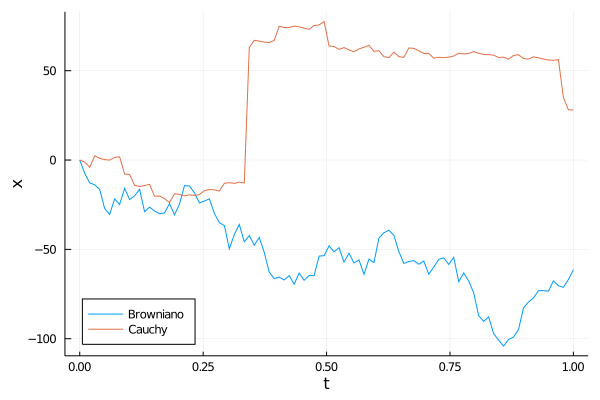
\includegraphics[width=0.4\textwidth]{figures/4_cauchy-brown.png}
    \caption{\scriptsize Processo di Brown e Processo di Cauchy a confronto \href{https://github.com/dodogabrie/Sistemi-Complessi/blob/master/python-project/lezione4/lez4_Cauchy-Brown.ipynb}{Link al codice in Julia}).}
    \label{fig:-fig}
\end{figure}

%%%%%%%%%%%%%%%%%%
%  Chapman form  %
%%%%%%%%%%%%%%%%%%
\subsection{Forma differenziale di C-K}%
\label{sub:Forma differenziale di Chapman - Kolmogorov}
Ipotizziamo di avere un processo stocastico Markoviano quindi per cui è possibile scrivere l'equazione di Chapman-Kolmogorov. Ipotizziamo che tale processo sia scomponibile\
\footnote{Ipotesi per cui si può scomporre sul Gardiner}  in una parte continua ed una non continua.\\
Si può dimostrare che un processo di questo tipo è descritto dalla seguente forma differenziale:
\begin{redbox}{Forma differenziale di Chapman - Kolmogorov}
    \begin{equation}
    \partial_{t}P(\vect{z},t| \vect{y}, t') = - \Gamma + \Phi
    \label{eq:4_CK}
    \end{equation}
\end{redbox}
\noindent
In cui $\Gamma$ è la parte contenente il processo continuo:
\[\begin{aligned}
    \Gamma = -\sum_{i}^{} \partial_{z_i}&\left[ A_i(\vect{z},t) P(\vect{z},t|\vect{y},t') \right] +\\
                         &+\sum_{i,J}^{} \frac{1}{2}\partial^2_{z_iZ_J}\left[ B_{iJ}(z,t) P(\vect{z},t|\vect{y},t') \right]
.\end{aligned}\]
Qui abbiamo un primo termine "deterministico" (con la $A$) che determina soltanto uno spostamento dell'oggetto ed un termine di diffusione (quello in $B$).\\
Nella $\Phi$ abbiamo invece il processo discontinuo:
\[\begin{aligned}
    \Phi = \int  d\vect{x} &\left[\omega (\vect{z}|\vect{x}, t) P(\vect{x},t|\vect{y}, t') \right. + \\
			   & \left. - \omega(\vect{x} | \vect{z}, t)  P(\vect{z},t|\vect{y},t') \right]
.\end{aligned}\]
Il termine $\Phi$ somiglia molto al termine della equazione di Volterra che abbiamo visto nella prima lezione (prob. di trovarsi in $\vect{z}$ è data dalla probabilità di finire in $\vect{z}$ da una posizione $\vect{x}$ diminuito la prob. di scappare in $\vect{x}$ dalla posizione $\vect{z}$).\\
La potenza della equazione è la sua generalità: se sappiamo che un processo è Markoviano (magari per la fisica che ci sta dietro) allora l'equazione di evoluzione delle prob. nel tempo sarà necessariamente quella sopra.
\begin{exmp}[$A=B=0$, quindi $\Gamma =0$]
    \[
        \partial_{t}P = \Phi
    .\] 
    Considerando il rapporto incrementale con passo $\Delta t$:
    \[
	P(z, t+\Delta t|y, t) = P(z,t|y,t) + \Delta t\cdot  \Phi
    .\] 
    Sfruttiamo la proprietà ovvia:
    \[
	P(\vect{z}, t|\vect{y}, t) = \delta (\vect{y}-\vect{z}) 
    .\] 
    Allora possiamo sviluppare $\Phi$ al primo ordine in $\Delta t$ l'espressione di $\Phi$ (in 1D):
    \[\begin{aligned}
	\Phi &= \int \omega (z|x, t) P(x,t|y,t') dx +\\
          & \qquad  - \int \omega (x|z, t) P(z,t|y,t') dx \simeq \\
	     & \simeq \int\left[\omega (z|x, t) \delta (x-y) - \omega (x|z, t)\delta (z-y) \right]dx = \\
	     & = \omega(z|y) - \delta(z-y) \int dx \omega(x|y)
    .\end{aligned}\]    
    \begin{greenbox}{Soluzione della forma diff. con termini continui}
    \begin{align}
	P&(z, t + \Delta t| y, t) = \nonumber \\
	&= \delta (z-y) \left[1-\Delta t\int dx \omega (x|z) \right] + \Delta t \cdot \omega (z|y) 
	\label{eq:forma_diff_cont}
    .\end{align}
    \end{greenbox}
    \noindent
    Riconosciamo nella equazione \ref{eq:forma_diff_cont} un primo termine (con la $\delta$) che corrisponde alla probabilità di essere già in $z$ diminuito della probabilità di andar via, il secondo termine ($\Delta t \omega (z|y)$) corrisponde invece alla probabilità di finire in $z$ arrivando da $y$.
    \noindent
\end{exmp}
\noindent

\clearpage
